\documentclass{article}
\usepackage[T1]{fontenc}
\usepackage[francais]{babel}

% Set page size and margins
% Replace `letterpaper' with`a4paper' for UK/EU standard size
\usepackage[a4paper,top=2cm,bottom=2cm,left=3cm,right=3cm,marginparwidth=1.75cm]{geometry}

% Useful packages
\usepackage{amsmath}
\usepackage{graphicx}

\usepackage{fancyhdr}
\pagestyle{fancy}

\usepackage{hyperref}
\hypersetup{
    colorlinks,
    citecolor=black,
    filecolor=black,
    linkcolor=black,
    urlcolor=black
}

\usepackage{glossaries}


\makenoidxglossaries


\loadglsentries{lexique}


%\renewcommand{\contentsname}{Table des matières}

\usepackage{xcolor}

\usepackage{eso-pic}
\usepackage{tikz}
\usepackage{float}

\usepackage{soul}
\usepackage{listings}
\newcommand{\hilight}{\makebox[0pt][s]{\color{green!50}\rule[-3.5pt]{1.0\linewidth}{11pt}}}


\usepackage{tikz}

\definecolor{mygray}{rgb}{0.5,0.5,0.5}
\lstdefinestyle{command}{
  backgroundcolor=\color{white},
  basicstyle=\ttfamily\color{black},
  keywordstyle=\color{blue},
  commentstyle=\color{mygray},
  stringstyle=\color{red},
  showstringspaces=false,
  upquote=true,
  morekeywords={sudo, ls, cd, mv, cp, rm, mkdir, chmod, chown, grep, find},
  captionpos=b,
  frame=single,
  numbers=left,
  numberstyle=\tiny\color{mygray},
  breaklines=true,
  breakatwhitespace=true,
  tabsize=2,
  keepspaces=true,
  caption={Linux Command},
  label=command,
}

\lstdefinestyle{cstyle}{
    language=C,
    basicstyle=\ttfamily,
    keywordstyle=\color{blue},
    commentstyle=\color{green!40!black},
    stringstyle=\color{red},
    identifierstyle=\color{black},
    numbers=left,
    numberstyle=\tiny\color{gray},
    frame=single,
    breaklines=true,
    showstringspaces=false,
    tabsize=4,
    morekeywords={int, char, void, if, else, while, for, return, typedef, struct, include},
    columns=flexible
}

\lstdefinestyle{makefilestyle}{
    language=make,
    basicstyle=\ttfamily,
    keywordstyle=\color{blue},
    commentstyle=\color{green!40!black},
    stringstyle=\color{red},
    identifierstyle=\color{black},
    numbers=left,
    numberstyle=\tiny\color{gray},
    frame=single,
    breaklines=true,
    showstringspaces=false,
    tabsize=4,
    morekeywords={ifeq, endif, else, ifdef, ifndef, define, endef, export, unexport, obj},
    columns=flexible
}

\bibliographystyle{plain} % We choose the "plain" reference style

\newcommand{\litmus}{LITMUS\textsuperscript{RT}}
\renewcommand{\epsilon}{\varepsilon} 
\renewcommand{\phi}{\varphi} 
\title{Rapport de stage Ingénieur \\-\\Implémentation d'un ordonnanceur temps réel sur
plateforme multi-cœur hétérogène\\-}
\author{BELPOIS Vincent}

\begin{document}

\date{2023}
\maketitle
\thispagestyle{empty}

\vspace{10mm}

\begin{center}
    
\includegraphics[width = 6cm]{Images/logo_ensma.png}
    \end{center}
    \vspace{2cm}
    \begin{center}
        
\includegraphics[width = 6cm]{Images/logo_LIAS.png}
    \end{center}
    \newpage
    \tableofcontents
    
    
    \AddToShipoutPictureBG{%
    \put(5,5){
\includegraphics[scale = 0.02]{Images/logo_ensma.png}}
    \put(90,5){
\includegraphics[scale = 0.08]{Images/logo_LIAS.png}}
    
    }
    \newpage
    
    \section*{Présentation du stage}
    \addcontentsline{toc}{section}{Présentation du stage}
    
    
    \subsection{Le L.I.A.S.}
    %Le LIAS c'est cool

    Parler des différentes équipes.
    Dans quelle équipe je suis ?
    \subsection{Le sujet du stage}
    
    Mon stage s'intéresse à l'implémentation d'un ordonanceur sur \gls{plateforme heterogene}\cite{bertout2020workload}

    Parler du projet SHRIMP. % en vrai faut que je me renseigne.

    \newpage
    \section[OS compatibles avec la carte]{Systèmes d'exploitation compatibles avec la carte ROCK960}
    \subsection{Présentation de la carte de développement}
    Le stage s'intéressant à l'implémentation d'un algorithme d'ordonnancement sur une plateforme hétérogène, une carte possédant un tel processeur est mis à ma disposition. Cette carte se nomme ROCK960 et est fabriquée par l'entreprise \textit{96Boards}. Cette carte de développement contient de nombreuses interfaces, mais nous nous contenteront d'utiliser l'interface série TTL. Nous nous connecterons à cette dernière via un convertisseur USB vers TTL. Cela permettra d'interfacer via un terminal qui fonctionnera avec une liaison série. 

\subsubsection{Le processeur RK3399}
Au centre de la carte est un \gls{SOC} Rockchip RK3399. Ce processeur contient deux type de cœurs, ou processeurs. Deux d'entre eux sont des processeurs Cortex-A72 et les quatre autres sont des processeurs Cortex-A53. Ces 6 processeurs utilisent le même jeu d'instruction : ARMv8-A 64-bit. Cela sera important par la suite afin de faciliter la migration de tâches entre les processeurs, en effet si les jeux d'instructions des processeurs étaient différents, plusieurs copies du code compilé devraient exister tout en maintenant un lien d'équivalence entre les deux codes. Cela est bien au delà de la portée de mon stage mais serait un point intéressant à explorer.

\begin{figure}[H]
    \centering
    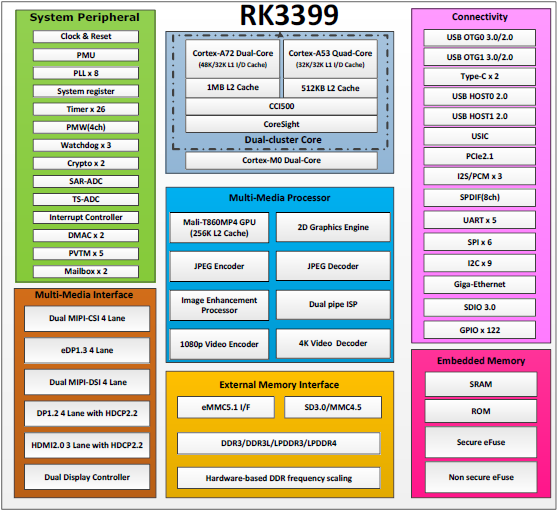
\includegraphics[width=0.45\paperwidth]{Images/RK3399_Block_Diagram.png}
    \caption{Architecture du processeur RK3399}
    \label{fig:archi_rk3399}
\end{figure}

Le SOC RK3399 contient bien d'autres composants et peut interfacer avec de nombreux périphériques (écran HDMI, USB, caméra MPI-CSI, SPI, UART, I2C, etc...) comme le montre la figure \ref{fig:archi_rk3399}. Ce diagramme nous montre aussi que les deux \gls{cluster} de processeurs ne partagent ni les caches L1 ni les caches L2, mais sont interconnectés par une interface CCI-500 qui, selon le site des développeurs ARM, permet la cohérence des caches des deux cluster.


\subsubsection{Interfacer avec la carte}

Comme mentionné précédement, la carte possède une sortie HDMI, mais nous nous contenterons d'utiliser l'interface série TTL. Nous nous connecterons à cette dernière via un convertisseur USB vers TTL. Cela permettra d'interfacer via un terminal qui fonctionnera avec une liaison série. J'ai utilisé l'utiitaire en ligne de commande \textit{minicom} pour me connecter à la carte. Pour que cela fonctionne, il faut configurer le \textit{baudrate} à une vitesse de 1M bauds, 8 bits de données, 1 bit de parité et 1 bit de stop (8N1).
La figure \ref{fig:terminal} montre le terminal série de \textit{minicom} connecté à la carte.


\begin{figure}[H]
    \centering
    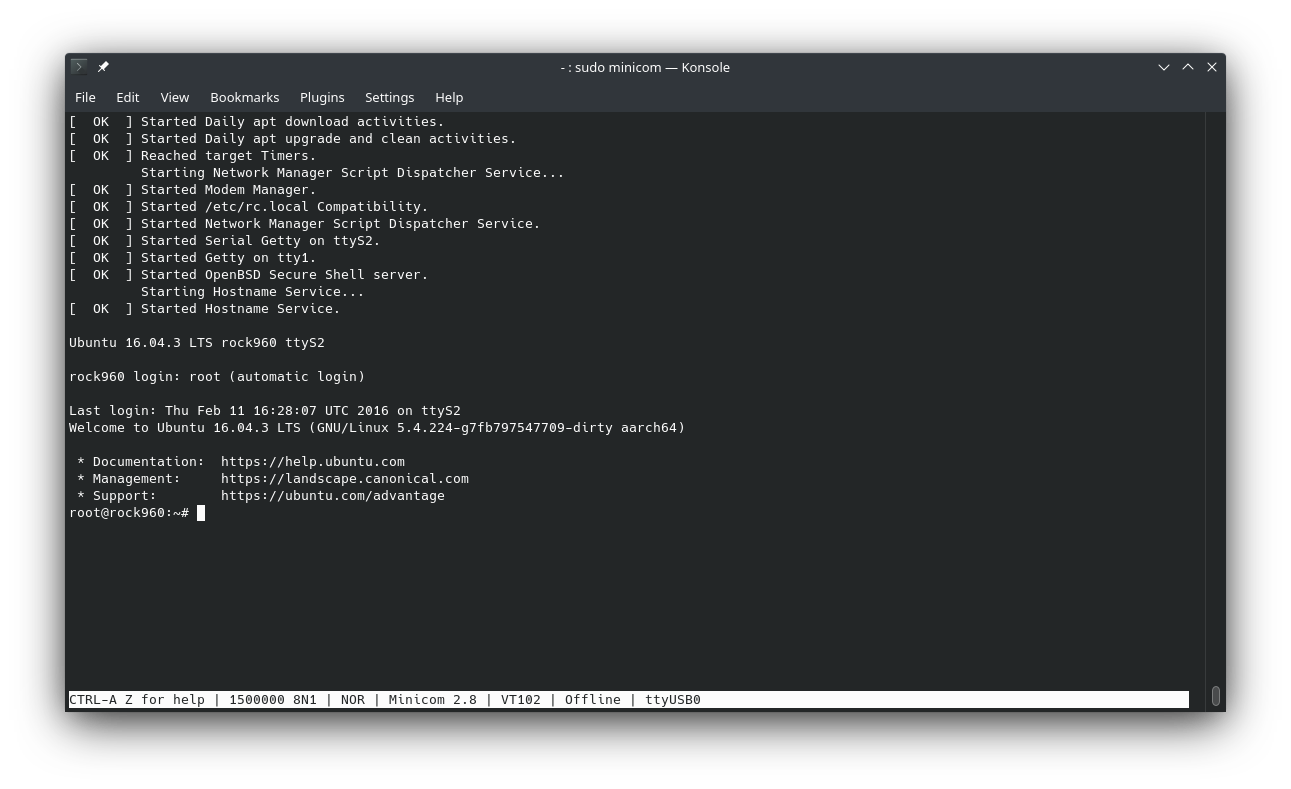
\includegraphics[width=0.75\textwidth]{Images/CaptureTerminalMinicom.png}
    \caption{Terminal série via minicom connecté à la carte}
    \label{fig:terminal}
\end{figure}



    \subsection{Installation d'un système d'exploitation}
    \subsubsection{Installation d'une image précompilée}

Pour premier tester l'Installation de linux sur la carte de développement, j'ai utilisé une image de la distribution Ubuntu fournie par le fabriquant 96Boards disponible sur leur site. Cette image se présente sous la forme d'une archive au format \texttt{.tar.gz}. Elle contient à la fois le \gls{bootloader}, le noyau Linux, et le système de fichier. Cette image (\texttt{system.img}) peut alors être gravée (ou \textit{flashée}) sur une carte micro SD. 

Depuis un terminal, en se déplaçant dans le dossier de l'archive extraite, on exécute la commande suivante : 
\begin{lstlisting}[style=command]
$ sudo dd if=system.img of=/dev/XXX bs=4M oflag=sync status=noxfer
\end{lstlisting}

\begin{center}
    \color{red}
    EXPLIQUER CE QUE FAIT CETTE COMMANDE \\
    Aussi dire en quoi on s'en servira dans des scripts afin d'accélérer le développement.
\end{center}


\subsubsection{Compilation de Linux depuis le code source}\label{sec:compilation-linux-source}

Ou est le code source linux ? Expliqué que j'étais déjà familié avec git et github pour des projets persos et tout.

Comment changer de version du code cloné. 

comment modifier quels modules sont chargés lors de la compilation de linux, interface graphique <-> fichier de config.
\subsubsection{Compilation croisée}

Toolchain : qu'est ce que c'est, de quoi elle est constituée ? Expliquer que l'on compile sur du x86 mais qu'on veut compiler pour du ARMv8xxx.

Variables d'environement? Qu'est ce que c'est sous linux, comparer a des 

Réalisation de scripts linux pour accélérer le développement. Que doit on charger pour charger le nouveau code compilé ?

Copy de l'image du noyau pour faire encore plus rapide.



    \subsection{Etude des versions de Linux compatibles}
    \subsection{Comment Linux gère le suport d'un processeur}

\subsection{Etude}

    


    
    \newpage
    \section{\litmus}
    
    \subsection{Présentation de \litmus}
    
    \subsection{Présentation de \textit{feather-trace}}
    
    \subsection{Implémentation d'un ordonanceur EDF partitioné}
    
    Le but du stage étant l'implémentation d'algorithmes d'ordonnancement sur plateforme hétérogène avec migration de tâches et de jobs entre les différent \gls{processeur}, il faudra être capable de réalise des \glspl{preemption} de jobs (une exécution de tâche), les migrer, assurer le traitement d'égalités et bien d'autre problèmes.


\subsubsection{Algorithme considéré}

On cherche alors, pour commencer, à implémenter un algorithme d'ordonnancement simple afin de se familiariser avec les méthodes et fonctions fourni par \litmus. J'ai donc choisi un algorithme partitionné pour la simplicité d'ordonnancement par \gls{processeur} que cela offre. Un algorithme EDF (\textit{Earliest Deadline First}) est alors choisi pour la simplicité du choix de la tâche a exécuter. Comme son nom l'indique, on choisi à chaque instant la tâche ayant l'échéance la plus proche. On nommera par la suite cet algorithme P-EDF (\textit{Partitionned Earliest Deadline First}).

Cet algorithme à aussi été choisi car il existe un tutoriel présent sur le site \href{https://litmus-rt.org}{litmus-rt.org} détaillant la plupart des fonctions nécessaires. 


Pour montrer le fonctionnement de cet algorithme, si l'on se place sur un même \gls{processeur}, on peut visualiser l'exécution de deux tâche periodiques : 
\begin{figure}[H]
    \center
    \begin{tikzpicture}[xscale=0.5, yscale=0.6]

        \newcommand\duration{15}
        \newcommand\TaskNum{2}

        % Define task properties

        \newcommand{\rectangles}[5]{
            \expandafter\def\csname rect#1ROW\endcsname{#2}
            \expandafter\def\csname rect#1START\endcsname{#3}
            \expandafter\def\csname rect#1END\endcsname{#4}
            \expandafter\def\csname rect#1COLOR\endcsname{#5}
        }

        \newcommand{\wakeup}[3]{
            \expandafter\def\csname wakeup#1ROW\endcsname{#2}
            \expandafter\def\csname wakeup#1TIME\endcsname{#3}
        }

        \newcommand{\deadlinee}[3]{
            \expandafter\def\csname deadline#1ROW\endcsname{#2}
            \expandafter\def\csname deadline#1TIME\endcsname{#3}
        }

        \newcommand{\execEnd}[3]{
            \expandafter\def\csname execEnd#1ROW\endcsname{#2}
            \expandafter\def\csname execEnd#1TIME\endcsname{#3}
        }
        
        
        
        \rectangles{0}{0}{0}{2}{"red"}
        \rectangles{1}{0}{5}{7}{"red"}
        \rectangles{2}{0}{10}{12}{"red"}
        
        \rectangles{3}{1}{2}{5}{"red"}
        \rectangles{4}{1}{7}{8}{"red"}
        
        
        
        \wakeup{0}{0}{0}
        \wakeup{1}{1}{0}
        \wakeup{4}{0}{5}

        \wakeup{5}{0}{5}
        \wakeup{2}{0}{5}
        \wakeup{3}{0}{10}

        \deadlinee{0}{0}{5}
        \deadlinee{1}{0}{5}
        \deadlinee{2}{0}{5}
        \deadlinee{3}{0}{10}
        \deadlinee{4}{0}{15}
        \deadlinee{5}{1}{15}

        \execEnd{0}{0}{2}
        \execEnd{1}{0}{7}
        \execEnd{2}{0}{12}
        \execEnd{3}{1}{8}        
        
        
        \foreach \rect in {0,...,4}{
            \pgfmathsetmacro{\row}{\csname rect\rect ROW\endcsname}
            \pgfmathsetmacro{\start}{\csname rect\rect START\endcsname}
            \pgfmathsetmacro{\end}{\csname rect\rect END\endcsname}
            \pgfmathsetmacro{\color}{\csname rect\rect COLOR\endcsname}

            \draw[fill=\color!30] (\start,1.5*\TaskNum - 0.5 - 1.5*\row) rectangle (\end,1.5*\TaskNum -1.5 - 1.5*\row) node[midway] {};
        }

        \foreach \wake in {0,...,5}{
            \pgfmathsetmacro{\row}{\csname wakeup\wake ROW\endcsname}
            \pgfmathsetmacro{\time}{\csname wakeup\wake TIME\endcsname}
            
            \draw[stealth-, thick] (\time,1.5*\TaskNum - 0.5 - 1.5*\row + 0.15) -- (\time,1.5*\TaskNum -1.5 - 1.5*\row) node[midway, left] {};
        }

        \foreach \dead in {0,...,5}{
            \pgfmathsetmacro{\row}{\csname deadline\dead ROW\endcsname}
            \pgfmathsetmacro{\time}{\csname deadline\dead TIME\endcsname}
            
            \draw[-stealth, thick] (\time,1.5*\TaskNum - 0.5 - 1.5*\row) -- (\time,1.5*\TaskNum -1.5 - 1.5*\row-0.15) node[midway, left] {};
        }

        \foreach \end in {0,...,3}{
            \pgfmathsetmacro{\row}{\csname execEnd\end ROW\endcsname}
            \pgfmathsetmacro{\time}{\csname execEnd\end TIME\endcsname}
            
            \draw[|-, thick] (\time,1.5*\TaskNum - 0.5 - 1.5*\row + 0.15) -- (\time,1.5*\TaskNum -1.5 - 1.5*\row) node[midway, left] {};
        }
        
        
        % Axes
        \draw[->] (0,0) -- (\duration + 1,0) node[right] {Temps};
        \draw[->] (0,0) -- (0,\TaskNum*1.5) node[above] {Taches};
        
        % Time ticks
        \foreach \x in {0,1,...,\duration}
            \draw (\x,0.1) -- (\x,-0.1) node[below] {\x};
        
            \node[left] at (-0.5,2) {$\tau_1(WCET=2,T=5)$};
            \node[left] at (-0.5,0.5) {$\tau_2(WCET=4,T=15)$};

    \end{tikzpicture}   
        
    \caption{Exemple de EDF à 2 tâches}
\end{figure}

On a ici une première tâche $\tau_1$ avec un pire temps d'exécution (\textit{Worst Case Execution Time}) de 2 et une période de 5, et une seconde tâche $\tau_2$ avec un pire temps d'exécution de 4 et une période de 15. On a alors préemption de la $\tau_2$ à $t=5$ afin d'exécuter $\tau_1$. Cela est dù au réveil de la tâche $\tau_1$ (représenté par la fleche montante), tâche qui est plus prioritaire que la tâche $\tau_2$ car l'échéance de la tâche $\tau_1$ est plus proche. 


\subsubsection{Implémentation}

La construction d'un plugin d'ordonnancement nécessite la déclaration d'un module au sens de Linux. Pour Linux un module est un élément de code qui peut être chargé dynamiquement lors de l'exécution du système d'exploitation. Un module permet alors d'étendre les fonctionnalités du noyau, il a donc ont accès aux fonctions du noyau, à ses ressources et peut aussi réaliser des appels systèmes.

Pour que notre nouvel ordonnanceur soit reconnu par le noyau Linux modifié (\litmus), il faut déclarer une fonction d'initialisation :
\begin{lstlisting}[style=cstyle]
#include <linux/module.h> // used for calling module_init()

static int __init init_p_edf(void)
{
    return 0; // indicates a successful initialisation
}

module_init(init_p_edf); // specify the entry point of the module 
\end{lstlisting} 

On peut alors enregistrer ce fichier sous le nom \lstinline{sched_p_edf.c} pour suivre la nomenclature des autres ordonnanceurs fournis avec avec \litmus. Ce fichier est enregistré dans le dossier \lstinline{llinux/litmus}. On peut alors modifier le fichier \lstinline{Makefile} de ce dossier afin de l'ajouter au fichier à compiler :

\begin{lstlisting}[style=makefilestyle]  
    obj-y = sched_p_edf.o
\end{lstlisting}    

On place notre fichier à compiler sous le mot-clé \texttt{obj-y} pour signifier que l'on veut ce module compilé et inclus lors de la compilation du noyau Linux.

Une fois le makefile modifié, la compilation de notre module sera exécutée lors de la compilation du noyau Linux à l'aide de make. La compilation du noyau est discutée dans la partie \ref{sec:compilation-linux-source}.

Il faut aussi déclarer un ensemble de fonctions propres à l'ordonnancement, comme pour l'admission de tâches, le réveil d'une tâche, la fin d'une tâche, le démarrage de l'ordonnanceur, etc. Voici l'ensemble des fonctions que j'ai déclaré pour mon ordonnanceur :
\newpage
\begin{lstlisting}[style=cstyle, caption={Déclaration des fonctions de l'ordonnanceur}, label={lst:decl-func-sched}]
static struct sched_plugin p_edf_plugin = {
    .plugin_name            = "P-EDF",
    .schedule               = p_edf_schedule,
    .task_wake_up           = p_edf_task_resume,
    .admit_task             = p_edf_admit_task,
    .task_new               = p_edf_task_new,
    .task_exit              = p_edf_task_exit,
    .get_domain_proc_info   = p_edf_get_domain_proc_info,
    .activate_plugin        = p_edf_activate_plugin,
    .deactivate_plugin      = p_edf_deactivate_plugin,
    .complete_job           = complete_job,
};
\end{lstlisting}

\litmus met à notre disposition un système d'abstraction pour ces fonctions afin que chaque ordonnanceur soit compatible avec les fonctions de \litmus.


\subsubsection{Résultats et essais}

Un algorithme partitionné nécessite le démarrage des tâches sur un processeur en particulier. Par exemple, j'ai ici démarré deux tâches \texttt{rtspin} avec \textit{liblitmus}. Les tâches \texttt{rtspin} sont des tâches dont la durée d'exécution est fixé et représente la condition de fin d'exécution de celle-ci.


Les deux tâches sont alors démarrées sur le processeur 3, comme en atteste le chiffre 3 dans les exécutions des tâches de la figure \ref{fig:edf-schedualibility-demo}L'une à un pire temps d'exécution de 2ms et une période de 5ms tandis que l'autre a un pire temps d'exécution de 4ms et une période de 7ms.

\begin{figure}[H]
    \centering
    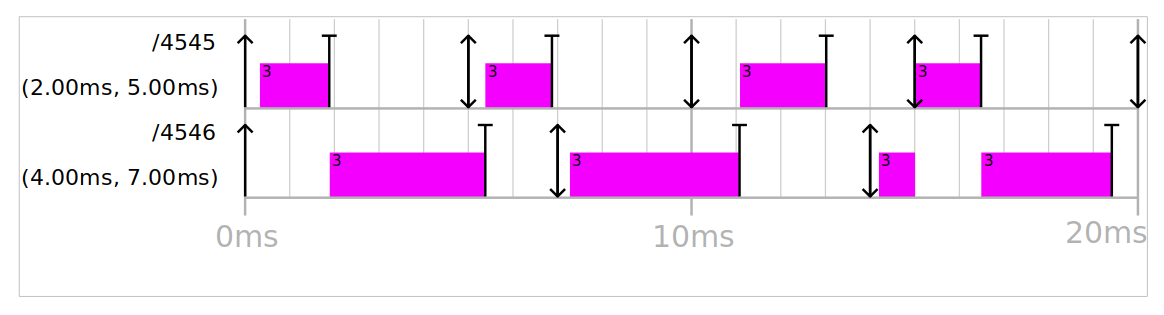
\includegraphics[width=0.95\textwidth]{Images/P-EDF-SCHEDUALIBILITY-DEMO.png}
    \caption{Ordonnancement de deux tâches avec P-EDF, toutes deux lancées sur le processeur 3}
    \label{fig:edf-schedualibility-demo}
\end{figure}

On peut voir qu'à $t=5ms$, il n'y a pas préemption de la première tâche et la seconde termine son exécution. En effet, selon EDF, la deuxième tâche à une \textit{deadline} dans 2ms, tandis que la première a une \textit{deadline} dans 5ms : la seconde est donc à cet instant plus prioritaire que la première. Cependant, à $t=15ms$, la seconde tâche est préemptée par la première car cette dernière se réveil et a une \textit{deadline} dans 5ms tandis que la seconde a une \textit{deadline} dans 6ms. On peut alors voir que la seconde tâche est préemptée à $t=15ms$ et reprend son exécution à $t=17ms$.

On remarque aussi que ce tracé n'étant pas théorique, des délais supplémentaires sont présents dù au coûts de préemption et de démarrage des tâches. On peut aussi voir que les deux tâches sont démarrées sur le même processeur, le processeur 3.
    
    
    
    \newpage
    \section*{Annexe}
    \addcontentsline{toc}{part}{Annexe}
    \begin{lstlisting}[style=makefilestyle, escapechar=\%, caption=linux/litmus/Makefile]
#
# Makefile for LITMUS^RT
#

obj-y = sched_plugin.o litmus.o \
        preempt.o \
        litmus_proc.o \
        budget.o \
        clustered.o \
        jobs.o \
        sync.o \
        rt_domain.o \
        edf_common.o \
        fp_common.o \
        fdso.o \
        locking.o \
        srp.o \
        bheap.o \
        binheap.o \
        ctrldev.o \
        uncachedev.o \
        sched_gsn_edf.o \
        sched_psn_edf.o \
        sched_pfp.o \
%\hilight%        sched_p_edf.o

obj-$(CONFIG_PLUGIN_CEDF) += sched_cedf.o
obj-$(CONFIG_PLUGIN_PFAIR) += sched_pfair.o

obj-$(CONFIG_FEATHER_TRACE) += ft_event.o ftdev.o
obj-$(CONFIG_SCHED_TASK_TRACE) += sched_task_trace.o
obj-$(CONFIG_SCHED_DEBUG_TRACE) += sched_trace.o
obj-$(CONFIG_SCHED_OVERHEAD_TRACE) += trace.o

obj-y += sched_pres.o

obj-y += reservations/
\end{lstlisting}


\begin{lstlisting}[style=cstyle, caption=linux/litmus/sched\_p\_edf.c, label=annexe:p-edf]
#include <linux/module.h>
#include <linux/percpu.h>
#include <linux/sched.h>
#include <litmus/litmus.h>
#include <litmus/budget.h>
#include <litmus/edf_common.h>
#include <litmus/jobs.h>
#include <litmus/litmus_proc.h>
#include <litmus/debug_trace.h>
#include <litmus/preempt.h>
#include <litmus/rt_domain.h>
#include <litmus/sched_plugin.h>
#include <litmus/sched_trace.h>

struct p_edf_cpu_state {
        rt_domain_t local_queues;
        int cpu;
        struct task_struct* scheduled;
};

static DEFINE_PER_CPU(struct p_edf_cpu_state, p_edf_cpu_state);

#define cpu_state_for(cpu_id)   (&per_cpu(p_edf_cpu_state, cpu_id))
#define local_cpu_state()       (this_cpu_ptr(&p_edf_cpu_state))
#define remote_edf(cpu)		(&per_cpu(p_edf_cpu_state, cpu).local_queues)
#define remote_pedf(cpu)	(&per_cpu(p_edf_cpu_state, cpu))
#define task_edf(task)		remote_edf(get_partition(task))

static struct domain_proc_info p_edf_domain_proc_info;

static long p_edf_get_domain_proc_info(struct domain_proc_info **ret)
{
        *ret = &p_edf_domain_proc_info;
        return 0;
}

static void p_edf_setup_domain_proc(void)
{
        int i, cpu;
        int num_rt_cpus = num_online_cpus();

        struct cd_mapping *cpu_map, *domain_map;

        memset(&p_edf_domain_proc_info, 0, sizeof(p_edf_domain_proc_info));
        init_domain_proc_info(&p_edf_domain_proc_info, num_rt_cpus, num_rt_cpus);
        p_edf_domain_proc_info.num_cpus = num_rt_cpus;
        p_edf_domain_proc_info.num_domains = num_rt_cpus;

        i = 0;
        for_each_online_cpu(cpu) {
                cpu_map = &p_edf_domain_proc_info.cpu_to_domains[i];
                domain_map = &p_edf_domain_proc_info.domain_to_cpus[i];

                cpu_map->id = cpu;
                domain_map->id = i;
                cpumask_set_cpu(i, cpu_map->mask);
                cpumask_set_cpu(cpu, domain_map->mask);
                ++i;
        }
}

/* This helper is called when task `prev` exhausted its budget or when
* it signaled a job completion. */
static void p_edf_job_completion(struct task_struct *prev, int budget_exhausted)
{
        sched_trace_task_completion(prev, budget_exhausted);
    TRACE_TASK(prev, "job_completion(forced=%d).\n", budget_exhausted);

    tsk_rt(prev)->completed = 0;
        /* Call common helper code to compute the next release time, deadline,
        * etc. */
        prepare_for_next_period(prev);
}

/* Add the task `tsk` to the appropriate queue. Assumes the caller holds the ready lock.
*/
static void p_edf_requeue(struct task_struct *tsk, struct p_edf_cpu_state *cpu_state)
{
        if (is_released(tsk, litmus_clock())) {
                /* Uses __add_ready() instead of add_ready() because we already
                    * hold the ready lock. */
                __add_ready(&cpu_state->local_queues, tsk);
                TRACE_TASK(tsk, "added to ready queue on reschedule\n");
        } else {
                /* Uses add_release() because we DON'T have the release lock. */
                add_release(&cpu_state->local_queues, tsk);
                TRACE_TASK(tsk, "added to release queue on reschedule\n");
        }
}

static int p_edf_check_for_preemption_on_release(rt_domain_t *local_queues)
{
        struct p_edf_cpu_state *state = container_of(local_queues, 
                                                struct p_edf_cpu_state,
                                                    local_queues);

        /* Because this is a callback from rt_domain_t we already hold
            * the necessary lock for the ready queue. */

        if (edf_preemption_needed(local_queues, state->scheduled)) {
                preempt_if_preemptable(state->scheduled, state->cpu);
                return 1;
        }
        return 0;
}

static long p_edf_activate_plugin(void)
{
        int cpu;
        struct p_edf_cpu_state *state;
        for_each_online_cpu(cpu) {
                TRACE("Initializing CPU%d...\n", cpu);
                state = cpu_state_for(cpu);
                state->cpu = cpu;
                state->scheduled = NULL;
                edf_domain_init(&state->local_queues,
                                p_edf_check_for_preemption_on_release,
                                NULL);
        }

        p_edf_setup_domain_proc();
        return 0;
}

static long p_edf_deactivate_plugin(void)
{
        destroy_domain_proc_info(&p_edf_domain_proc_info);
        return 0;
}



static struct task_struct* p_edf_schedule(struct task_struct * prev)
{
        struct p_edf_cpu_state *local_state = local_cpu_state();

        /* next == NULL means "schedule background work". */
        struct task_struct *next = NULL;

        /* prev's task state */
        int exists, out_of_time, job_completed, self_suspends, preempt, resched;

        raw_spin_lock(&local_state->local_queues.ready_lock);

        BUG_ON(local_state->scheduled && local_state->scheduled != prev);
        BUG_ON(local_state->scheduled && !is_realtime(prev));

        exists = local_state->scheduled != NULL;
        self_suspends = exists && !is_current_running();
        out_of_time = exists && budget_enforced(prev) && budget_exhausted(prev);
        job_completed = exists && is_completed(prev);

        /* preempt is true if task `prev` has lower priority than something on
        * the ready queue. */
        preempt = edf_preemption_needed(&local_state->local_queues, prev);

        /* check all conditions that make us reschedule */
        resched = preempt;

        /* if `prev` suspends, it CANNOT be scheduled anymore => reschedule */
        if (self_suspends) {
                resched = 1;
        }

        /* also check for (in-)voluntary job completions */
        if (out_of_time || job_completed) {
                p_edf_job_completion(prev, out_of_time);
                resched = 1;
        }

        if (resched) {
                /* First check if the previous task goes back onto the ready
                * queue, which it does if it did not self_suspend.
                */
                if (exists && !self_suspends) {
                        p_edf_requeue(prev, local_state);
                }
                next = __take_ready(&local_state->local_queues);
        } else {
                /* No preemption is required. */
                next = local_state->scheduled;
        }

        local_state->scheduled = next;
        if (exists && prev != next) {
                TRACE_TASK(prev, "descheduled.\n");
        }
        if (next) {
                TRACE_TASK(next, "scheduled.\n");
        }

        /* This mandatory. It triggers a transition in the LITMUS^RT remote
        * preemption state machine. Call this AFTER the plugin has made a
        * local scheduling decision.
        */
        sched_state_task_picked();

        raw_spin_unlock(&local_state->local_queues.ready_lock);
        return next;
}

static long p_edf_admit_task(struct task_struct *tsk)
{
        if (task_cpu(tsk) == get_partition(tsk)) {
                TRACE_TASK(tsk, "accepted by p_edf plugin.\n");
                return 0;
        }
        return -EINVAL;
}

static void p_edf_task_new(struct task_struct *tsk, int on_runqueue,
                            int is_running)
{
        /* We'll use this to store IRQ flags. */
        unsigned long flags;
        struct p_edf_cpu_state *state = cpu_state_for(get_partition(tsk));
        lt_t now;

        TRACE_TASK(tsk, "is a new RT task %llu (on runqueue:%d, running:%d)\n",
                    litmus_clock(), on_runqueue, is_running);

        /* Acquire the lock protecting the state and disable interrupts. */
        raw_spin_lock_irqsave(&state->local_queues.ready_lock, flags);

        now = litmus_clock();

        /* Release the first job now. */
        release_at(tsk, now);

        if (is_running) {
                /* If tsk is running, then no other task can be running
                    * on the local CPU. */
                BUG_ON(state->scheduled != NULL);
                state->scheduled = tsk;
        } else if (on_runqueue) {
                p_edf_requeue(tsk, state);
        }

        if (edf_preemption_needed(&state->local_queues, state->scheduled))
                preempt_if_preemptable(state->scheduled, state->cpu);

        raw_spin_unlock_irqrestore(&state->local_queues.ready_lock, flags);
}

static void p_edf_task_exit(struct task_struct *tsk)
{
        unsigned long flags;
        struct p_edf_cpu_state *state = cpu_state_for(get_partition(tsk));
        raw_spin_lock_irqsave(&state->local_queues.ready_lock, flags);
        rt_domain_t*		edf;

        /* For simplicity, we assume here that the task is no longer queued anywhere else. This
            * is the case when tasks exit by themselves; additional queue management is
            * is required if tasks are forced out of real-time mode by other tasks. */
        
        if (is_queued(tsk)){
                edf = task_edf(tsk);
                remove(edf,tsk);
        }

        if (state->scheduled == tsk) {
                state->scheduled = NULL;
        }
        
        preempt_if_preemptable(state->scheduled, state->cpu);
        raw_spin_unlock_irqrestore(&state->local_queues.ready_lock, flags);
}

/* Called when the state of tsk changes back to TASK_RUNNING.
    * We need to requeue the task.
    *
    * NOTE: If a sporadic task is suspended for a long time,
    * this might actually be an event-driven release of a new job.
    */
static void p_edf_task_resume(struct task_struct  *tsk)
{
        unsigned long flags;
        struct p_edf_cpu_state *state = cpu_state_for(get_partition(tsk));
        lt_t now;
        TRACE_TASK(tsk, "wake_up at %llu\n", litmus_clock());
        raw_spin_lock_irqsave(&state->local_queues.ready_lock, flags);

        now = litmus_clock();

        if (is_sporadic(tsk) && is_tardy(tsk, now)) {
                /* This sporadic task was gone for a "long" time and woke up past
                    * its deadline. Give it a new budget by triggering a job
                    * release. */
                inferred_sporadic_job_release_at(tsk, now);
                TRACE_TASK(tsk, "woke up too late.\n");
        }

        /* This check is required to avoid races with tasks that resume before
            * the scheduler "noticed" that it resumed. That is, the wake up may
            * race with the call to schedule(). */
        if (state->scheduled != tsk) {
                TRACE_TASK(tsk, "is being reqeued\n");
                p_edf_requeue(tsk, state);
                if (edf_preemption_needed(&state->local_queues, state->scheduled)) {
                        preempt_if_preemptable(state->scheduled, state->cpu);
                }
        }

        raw_spin_unlock_irqrestore(&state->local_queues.ready_lock, flags);
}


static struct sched_plugin p_edf_plugin = {
        .plugin_name            = "P-EDF",
        .schedule               = p_edf_schedule,
        .task_wake_up           = p_edf_task_resume,
        .admit_task             = p_edf_admit_task,
        .task_new               = p_edf_task_new,
        .task_exit              = p_edf_task_exit,
        .get_domain_proc_info   = p_edf_get_domain_proc_info,
        .activate_plugin        = p_edf_activate_plugin,
        .deactivate_plugin      = p_edf_deactivate_plugin,
        .complete_job           = complete_job,
};

static int __init init_p_edf(void)
{
        return register_sched_plugin(&p_edf_plugin);
}

module_init(init_p_edf);     
\end{lstlisting}

\begin{lstlisting}[style=config, caption=Partie du fichier .config liée a \litmus]
# LITMUS^RT
#

#
# Scheduling
#
CONFIG_PLUGIN_PFAIR=y
# CONFIG_RELEASE_MASTER is not set
CONFIG_PREFER_LOCAL_LINKING=y
CONFIG_LITMUS_QUANTUM_LENGTH_US=1000
CONFIG_BUG_ON_MIGRATION_DEADLOCK=y
# end of Scheduling

#
# Real-Time Synchronization
#
CONFIG_NP_SECTION=y
CONFIG_LITMUS_LOCKING=y
# end of Real-Time Synchronization

#
# Performance Enhancements
#
CONFIG_ALLOW_EARLY_RELEASE=y
# CONFIG_EDF_TIE_BREAK_LATENESS is not set
CONFIG_EDF_TIE_BREAK_LATENESS_NORM=y
# CONFIG_EDF_TIE_BREAK_HASH is not set
# CONFIG_EDF_PID_TIE_BREAK is not set
# end of Performance Enhancements

#
# Tracing
#
CONFIG_FEATHER_TRACE=y
CONFIG_SCHED_TASK_TRACE=y
CONFIG_SCHED_TASK_TRACE_SHIFT=9
CONFIG_SCHED_OVERHEAD_TRACE=y
CONFIG_SCHED_OVERHEAD_TRACE_SHIFT=22
CONFIG_SCHED_DEBUG_TRACE=y
CONFIG_SCHED_DEBUG_TRACE_SHIFT=18
CONFIG_SCHED_DEBUG_TRACE_CALLER=y
# CONFIG_PREEMPT_STATE_TRACE is not set
# CONFIG_REPORT_TIMER_LATENCY is not set
# end of Tracing
# end of LITMUS^RT
\end{lstlisting}


\begin{lstlisting}[style=cstyle, escapechar=\%, caption=Modifications apportées au fichier \texttt{rk3399.dtsi}, label=annexe:cache]
cpus {
        #address-cells = <2>;
        #size-cells = <0>;

        cpu-map {
                cluster0 {
                        core0 {
                                cpu = <&cpu_l0>;
                        };
                        core1 {
                                cpu = <&cpu_l1>;
                        };
                        core2 {
                                cpu = <&cpu_l2>;
                        };
                        core3 {
                                cpu = <&cpu_l3>;
                        };
                };

                cluster1 {
                        core0 {
                                cpu = <&cpu_b0>;
                        };
                        core1 {
                                cpu = <&cpu_b1>;
                        };
                };
        };

        cpu_l0: cpu@0 {
                device_type = "cpu";
                compatible = "arm,cortex-a53";
                reg = <0x0 0x0>;
                enable-method = "psci";
%\hilight%                next-level-cache = <&l2_0>;
                capacity-dmips-mhz = <485>;
                clocks = <&cru ARMCLKL>;
                #cooling-cells = <2>; /* min followed by max */
                dynamic-power-coefficient = <100>;
                cpu-idle-states = <&CPU_SLEEP &CLUSTER_SLEEP>;

%\hilight%                l2_0: l2-cache {
%\hilight%                compatible = "cache,arm,arch-cache";
%\hilight%        };
        };

        cpu_l1: cpu@1 {
                device_type = "cpu";
                compatible = "arm,cortex-a53";
                reg = <0x0 0x1>;
                enable-method = "psci";
%\hilight%                next-level-cache = <&l2_0>;
                capacity-dmips-mhz = <485>;
                clocks = <&cru ARMCLKL>;
                #cooling-cells = <2>; /* min followed by max */
                dynamic-power-coefficient = <100>;
                cpu-idle-states = <&CPU_SLEEP &CLUSTER_SLEEP>;
        };

        cpu_l2: cpu@2 {
                device_type = "cpu";
                compatible = "arm,cortex-a53";
                reg = <0x0 0x2>;
                enable-method = "psci";
%\hilight%                next-level-cache = <&l2_0>;
                capacity-dmips-mhz = <485>;
                clocks = <&cru ARMCLKL>;
                #cooling-cells = <2>; /* min followed by max */
                dynamic-power-coefficient = <100>;
                cpu-idle-states = <&CPU_SLEEP &CLUSTER_SLEEP>;
        };

        cpu_l3: cpu@3 {
                device_type = "cpu";
                compatible = "arm,cortex-a53";
                reg = <0x0 0x3>;
                enable-method = "psci";
%\hilight%                next-level-cache = <&l2_0>;
                capacity-dmips-mhz = <485>;
                clocks = <&cru ARMCLKL>;
                #cooling-cells = <2>; /* min followed by max */
                dynamic-power-coefficient = <100>;
                cpu-idle-states = <&CPU_SLEEP &CLUSTER_SLEEP>;
        };

        cpu_b0: cpu@100 {
                device_type = "cpu";
                compatible = "arm,cortex-a72";
                reg = <0x0 0x100>;
                enable-method = "psci";
                next-level-cache = <&l2_1>;
                capacity-dmips-mhz = <1024>;
                clocks = <&cru ARMCLKB>;
                #cooling-cells = <2>; /* min followed by max */
                dynamic-power-coefficient = <436>;
                cpu-idle-states = <&CPU_SLEEP &CLUSTER_SLEEP>;
                
%\hilight%                l2_1: l2-cache {
%\hilight%                compatible = "cache,arm,arch-cache";
%\hilight%        };
        };

        cpu_b1: cpu@101 {
                device_type = "cpu";
                compatible = "arm,cortex-a72";
                reg = <0x0 0x101>;
                enable-method = "psci";
%\hilight%                next-level-cache = <&l2_1>;
                capacity-dmips-mhz = <1024>;
                clocks = <&cru ARMCLKB>;
                #cooling-cells = <2>; /* min followed by max */
                dynamic-power-coefficient = <436>;
                cpu-idle-states = <&CPU_SLEEP &CLUSTER_SLEEP>;
        };
        ...
}
\end{lstlisting}

    \newpage
    \bibliography{refs} % Entries are in the refs.bib file
    \newpage
    \listoffigures
    
    \printnoidxglossaries
\end{document}
    